\newpage
\section{mips Processor}
	A computer architecture is defined by it's instruction set and architectural state. The architectural state for the MIPS processor consists of the program counter and the 32 registers. We only consider the following instruction set:\\ R-type arithmetic/logic instructions: add, sub, and, or, slt.\\
	Memory instructions: lw, sw\\
	Branches: beq\\
	After having built the microarchitectures with these instructions we extend them with addi and j.\\
	We will divide our microarchitectures into two interacting parts: the datapath and the control. The datapath operates on words of data. It contains structures such as memories, registers, ALUs, and multiplexers. MIPS is a 32-bit architecture, so we will use a 32-bit datapath. The control unit receives the current instruction from the datapath and tells the datapath how to execute that instruction. Specifically, the control unit produces multiplexer select, register enable, and memory write signals to control the operation of the datapath.\\
	It is often good to seperate the memory into two, one containing the instructions and the other the data.\\
	The microprocessor is built of clocked state elements and combinational logic, so it too is a synchronous sequential circuit. Indeed, the processor can be viewed as a giant finite state machine, or as a collection of simpler interacting state machines.\\
	\subsection{Execution time}
	The execution time for a program is given by:
	\begin{equation}
		T= (\#instructions)*(\frac{cycles}{instruction})(\frac{seconds}{cycle})
	\end{equation}
	\subsection{Different architectures}
		\subsubsection{Singel-sycle}
			Executes an entire instruction in one cycle. It is easy to explain and has a simple control unit. Because it completes the operation in one cycle, it does not require any nonarchitectural state. However, the cycle time is limited by the slowest instruction.
			\begin{center}
				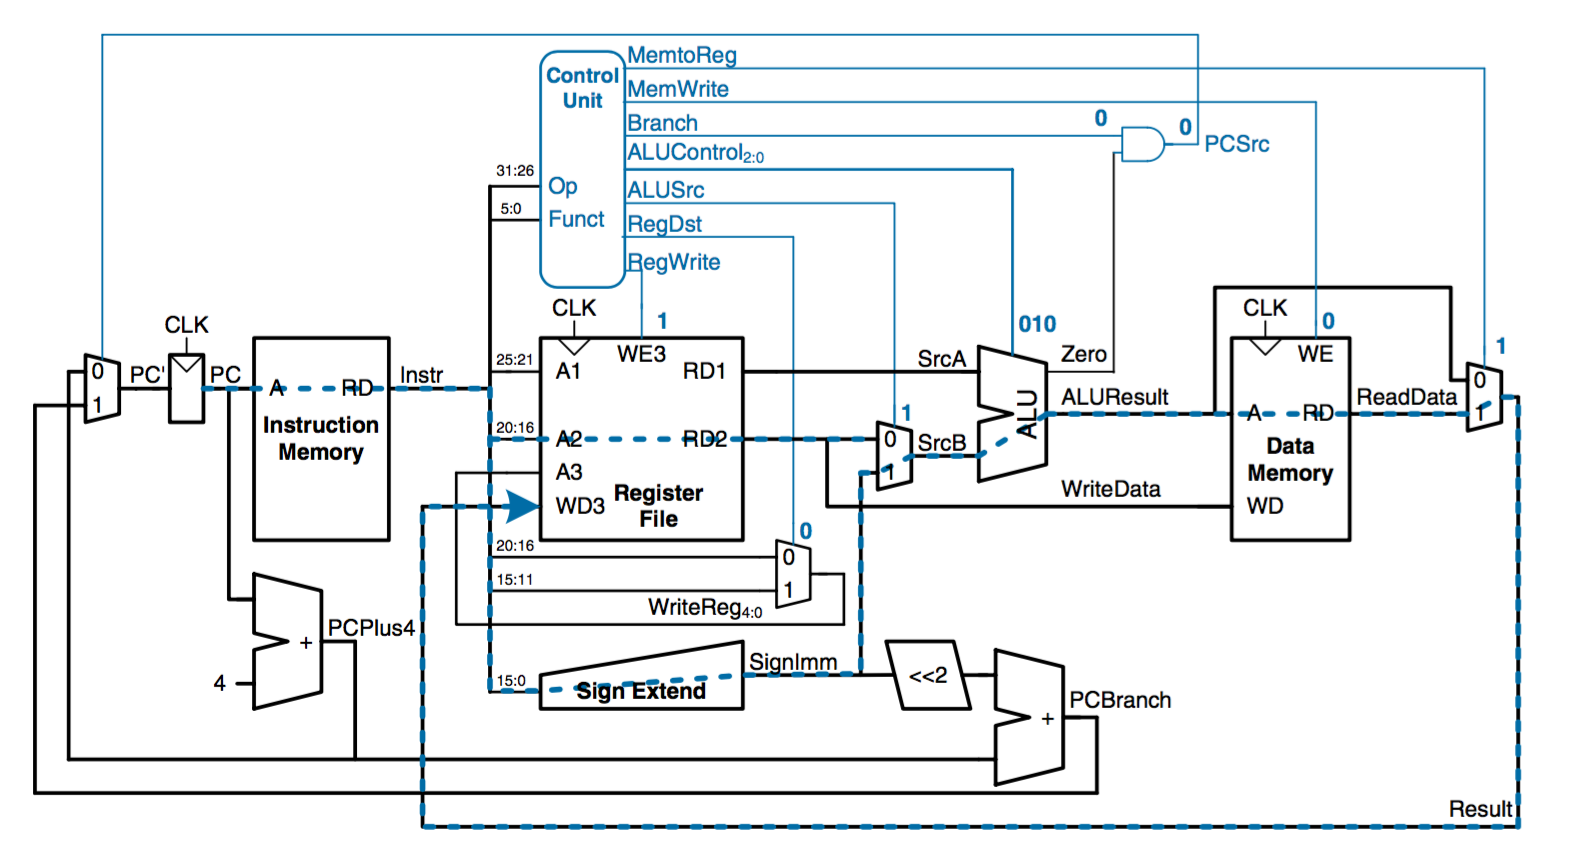
\includegraphics[width = 15cm]{images/single.png}
			\end{center}
			\paragraph{Performance}
			\begin{equation}
				T_c = T_{pcq_PC} + 2*t_{mem} + t_{RFread} + 2*t_{mux} + t_{ALU} + t_{RFsetup}
			\end{equation}
			\paragraph{Problems}
				The single cycle has 3 major problems:
				\begin{enumerate}
					\item requires a clock cycle long enough to support the slowest instruction (lw)
					\item requires 3 adders which are expensive
					\item Has two memories one for instructions and one for data. Most computers have one.
				\end{enumerate}
		\subsubsection{Multicycle}
			executes instructions in a series of shorter cycles. In each short step, the processor can read or write the memory or register file or use the ALU. Simpler instructions execute in fewer cycles than complicated ones. Moreover, the multicycle microarchitecture reduces the hardware cost by reusing expensive hardware blocks such as adders and memories(has one adder and one memory). The multicycle microprocessor accomplishes this by adding several nonarchitectural registers to hold intermediate results. The multicycle processor executes only one instruction at a time, but each instruction takes multiple clock cycles. The controller produces different signals on different steps during execution of a single instruction, so it is now a finite state machine rather than combinational logic.
			\begin{center}
				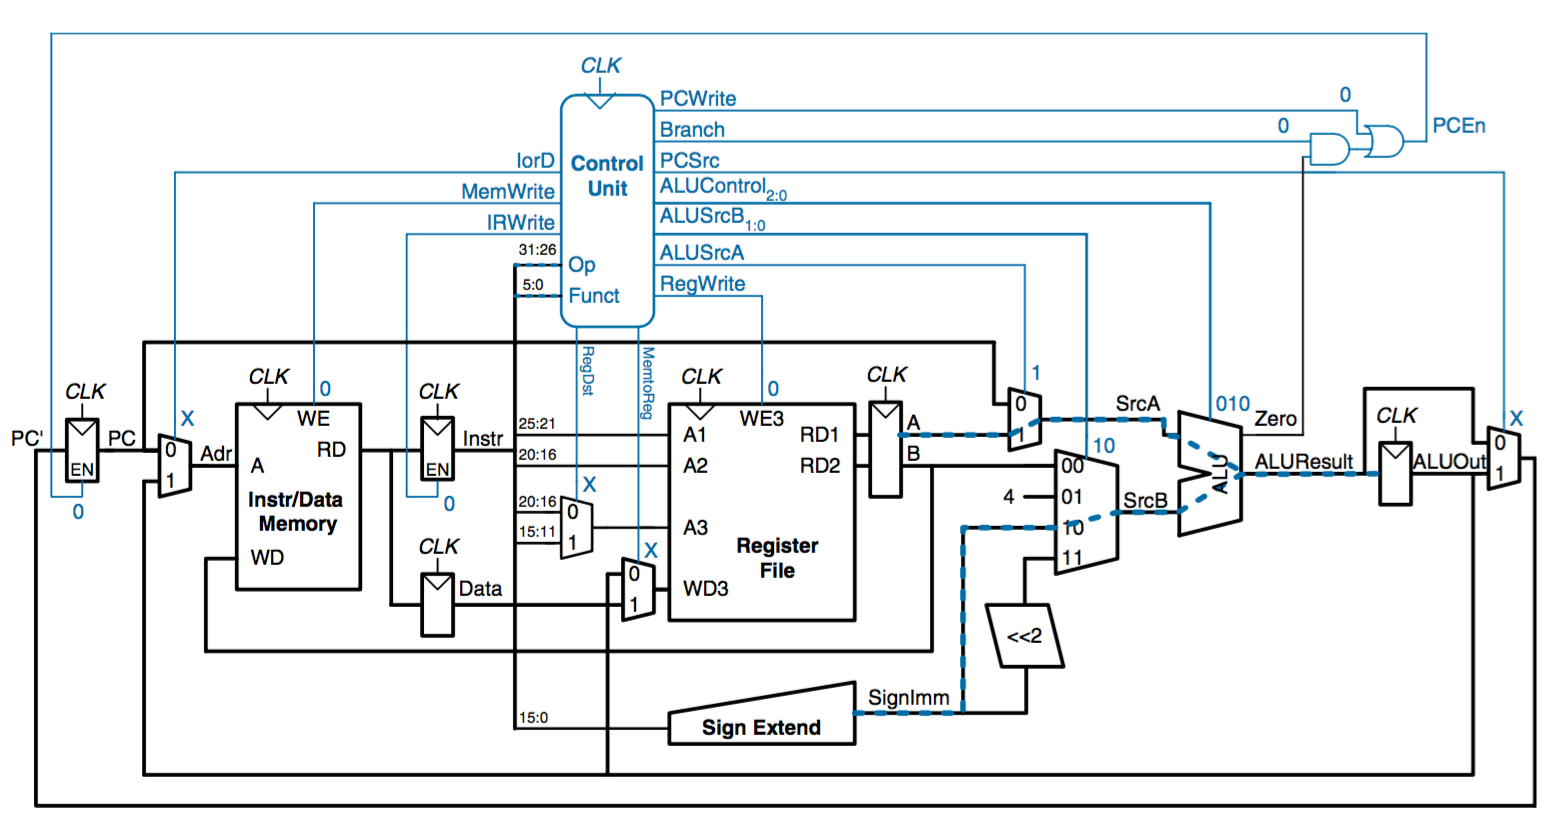
\includegraphics[width = 15cm]{images/multi}
			\end{center}
			\paragraph{Performance}
			The multicycle processor requires three cycles for beq and j instruc- tions, four cycles for sw, addi, and R-type instructions, and five cycles for lw instructions. The CPI depends on the relative likelihood that each instruction is used.
			\begin{equation}
				T_c = T_{pcq} + t_{mux} + MAX(t_{ALU}+ t_{mux}, t_{mem})+ t_{setup}
			\end{equation}
		\subsubsection{Pipeline}
			applies pipelining to the single-cycle microarchitecture. It therefore can execute several instructions simultaneously, improving the throughput significantly. Pipelining must add logic to handle dependencies between simultaneously executing instructions. It also requires nonarchitectural pipeline registers. The added logic and registers are worthwhile; all commercial high-performance processors use pipelining today.\\
			We design a pipelined processor by sub- dividing the single-cycle processor into five pipeline stages. Thus, five instructions can execute simultaneously, one in each stage. Because each stage has only one-fifth of the entire logic, the clock frequency is almost five times faster. Hence, the latency of each instruction is ideally unchanged, but the throughput is ideally five times better. Microprocessors execute millions or billions of instructions per second, so throughput is more important than latency.  Pipelining introduces some overhead, so the throughput will not be quite as high as we might ideally desire.\\
			Reading and writing the memory and register file and using the ALU typically constitute the biggest delays in the processor. We choose five pipeline stages so that each stage involves exactly one of these slow steps. Specifically, we call the five stages Fetch, Decode, Execute, Memory, and Writeback. They are similar to the five steps that the multicycle processor used to perform lw. In the Fetch stage, the processor reads the instruction from instruction memory. In the Decode stage, the processor reads the source operands from the register file and decodes the instruction to produce the control signals. In the Execute stage, the processor performs a computation with the ALU. In the Memory stage, the processor reads or writes data memory. Finally, in the Writeback stage, the processor writes the result to the register file, when applicable.
			\begin{center}
				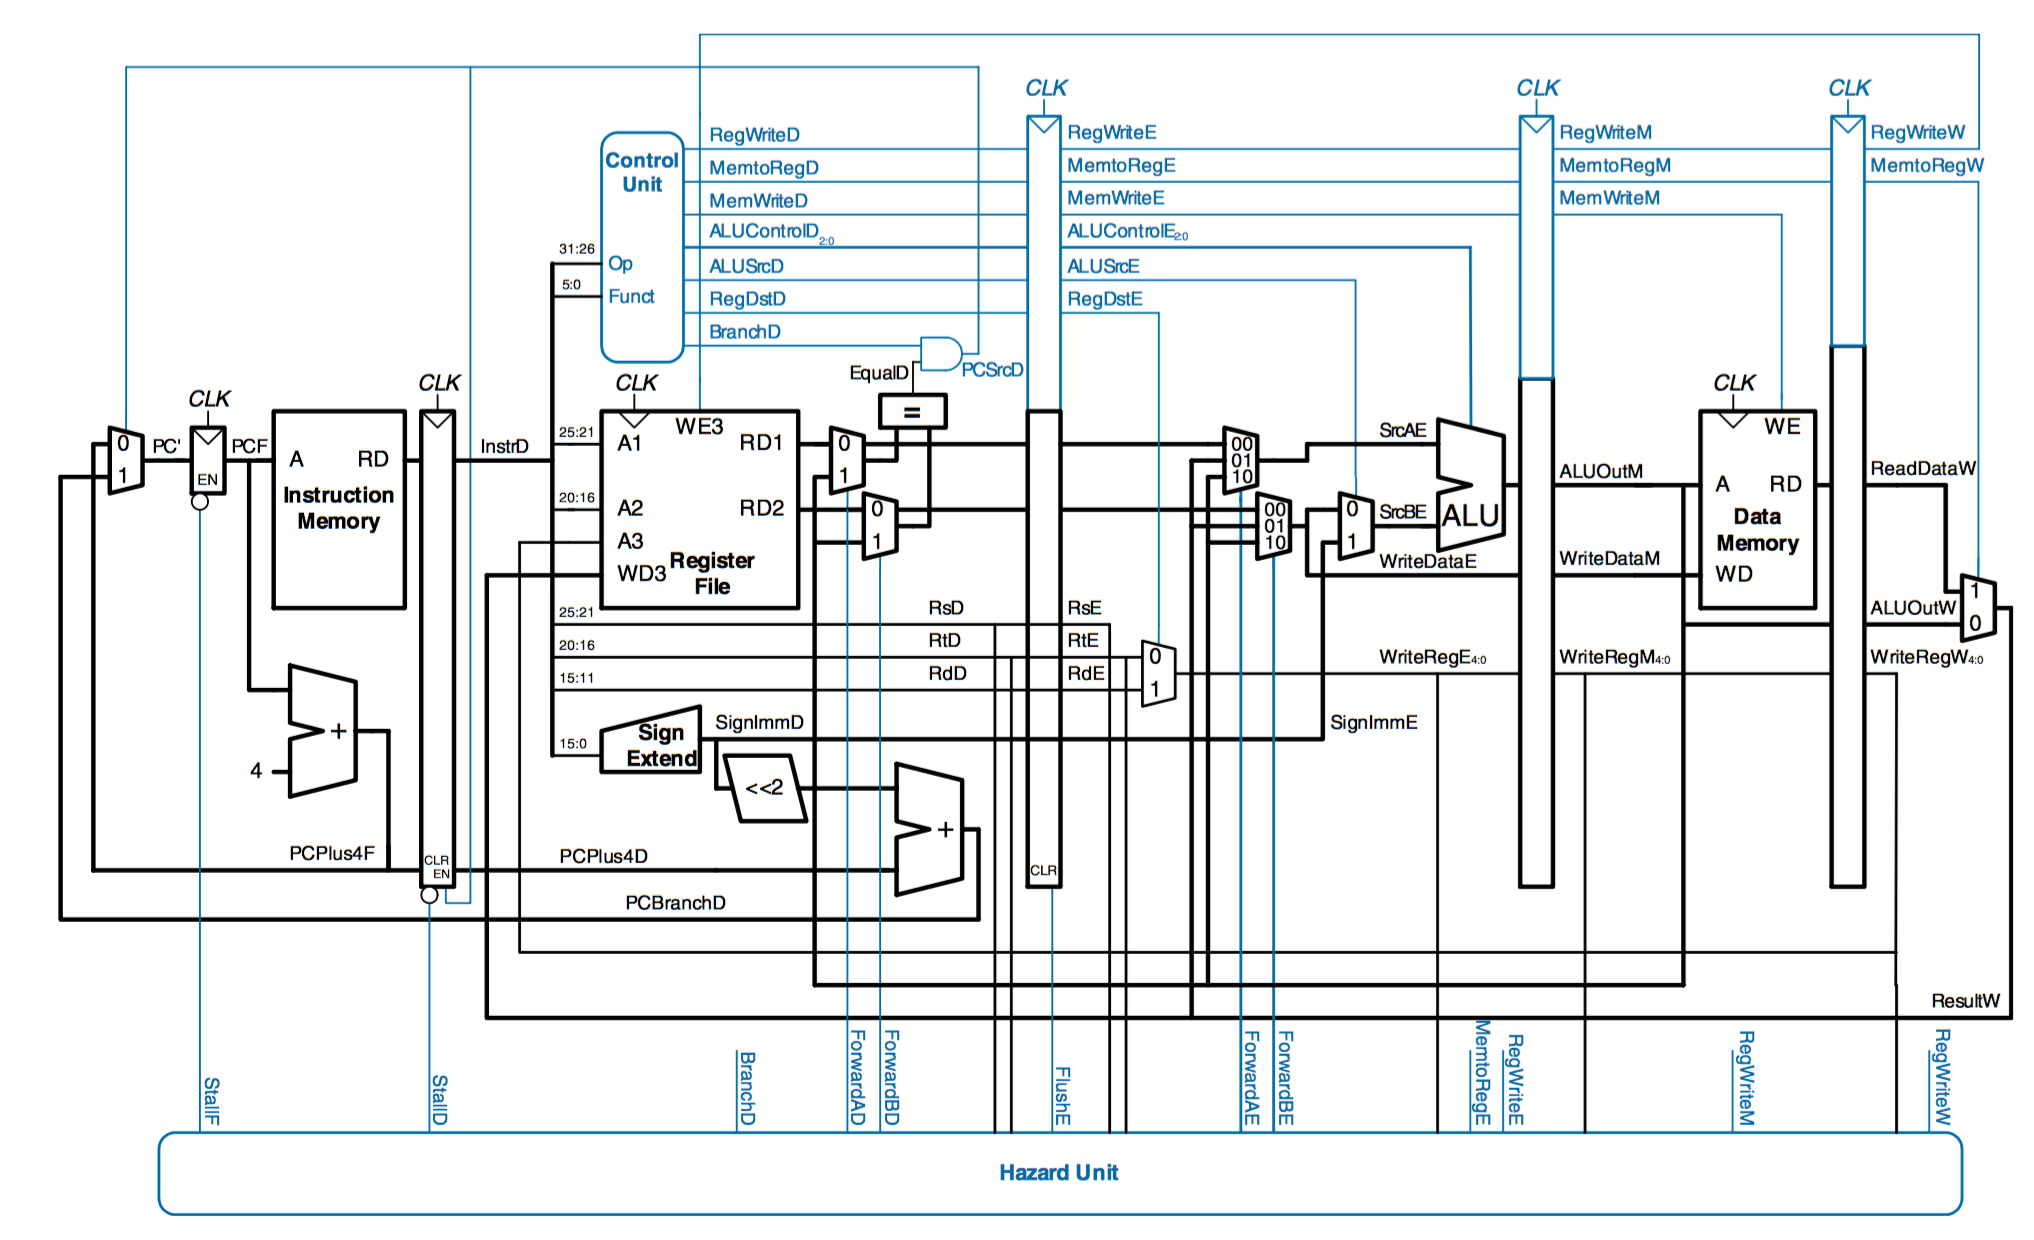
\includegraphics[width = 15cm]{images/pipeline}
			\end{center}
			\paragraph{Hazards}
				Hazards are classified as data hazards or control hazards. A data hazard occurs when an instruction tries to read a register that has not yet been written back by a previous instruction. A control hazard occurs when the decision of what instruction to fetch next has not been made by the time the fetch takes place. This can kind of be fixed with the hazard detection unit(by forwarding). They can also be solved by stalling the pipeline. stalling a stage is performed by disabling the pipeline register, so that the contents do not change. When a stage is stalled, all previous stages must also be stalled, so that no subsequent instructions are lost. Stalls degrade performance.
			\paragraph{Performance}
				CPI should idealy be 1, but a stall or a flush waste a cycle.


















